% =====================================================================
%  Plantilla profesional y compacta (límite: 4 páginas)
% =====================================================================
\documentclass[11pt,a4paper]{article}

% --------------------------- Idioma / codificación ---------------------------
\usepackage[english]{babel}
\usepackage[utf8]{inputenc}
\usepackage[T1]{fontenc}
\usepackage{lmodern}

% --------------------------- Página y márgenes ---------------------------
\usepackage[a4paper,margin=2.3cm,top=2.1cm,bottom=2.3cm]{geometry}
\usepackage{setspace}
\setstretch{1.04}

% --------------------------- Color corporativo ---------------------------
\usepackage{xcolor}
\definecolor{accent}{HTML}{0B5394}  
\definecolor{accentlight}{HTML}{E8F0FA}
\definecolor{greytext}{HTML}{555555}

% --------------------------- Tipografía de secciones ---------------------------
\usepackage{titlesec}
\titleformat{\section}
  {\large\bfseries\color{accent}}
  {\thesection.}{0.5em}{}
\titlespacing{\section}{0pt}{1.3em plus 1em minus 0.4em}{0.6em}

\titleformat{\subsection}
  {\normalsize\bfseries\color{accent!80!black}}
  {\thesubsection.}{0.5em}{}
\titlespacing{\subsection}{0pt}{1em plus 0.6em minus 0.3em}{0.4em}

% --------------------------- Cabecera / pie de página ---------------------------
\usepackage{fancyhdr}
\pagestyle{fancy}
\fancyhf{}
\renewcommand{\headrulewidth}{0.4pt}
\renewcommand{\footrulewidth}{0pt}
\fancyhead[L]{\small\color{greytext}Ejercicio 1 --- NoThrust Inc.}
\fancyhead[R]{\small\color{greytext}Programación y Prototipado}
\fancyfoot[C]{\small\color{greytext}\thepage\ / \pageref{LastPage}}
\usepackage{lastpage}

% --------------------------- Figuras, tablas, enlaces ---------------------------
\usepackage{graphicx}
\usepackage{caption}
\usepackage{float}
\usepackage{xltabular}
\usepackage{booktabs}
\usepackage[hidelinks,colorlinks=true,linkcolor=accent,citecolor=accent,urlcolor=accent]{hyperref}
\usepackage{enumitem}
\setlist{itemsep=0.15em, topsep=0.3em}

% --------------------------- Datos del documento ---------------------------
\newcommand{\miTitulo}{Integrated software solution for NoThrust Inc.}
\newcommand{\miSubtitulo}{Selected phase: \emph{Analysis}}
\newcommand{\miAutor}{Nicolás Rey Alonso}
\newcommand{\miAsignatura}{Programación y Prototipado --- SIANI}

\begin{document}

% =====================================================================
% BLOQUE DE TÍTULO (compacto, sin página aparte, para ahorrar espacio)
% =====================================================================
\begin{center}
  {\LARGE\bfseries\color{accent} \miTitulo\par}
  \vspace{0.3em}
  {\large\color{greytext} \miSubtitulo\par}
  \vspace{0.6em}
  {\normalsize \miAutor \;\textbar\; \miAsignatura \;\textbar\; \today\par}
\end{center}

\vspace{0.3em}
{\color{accent}\hrule height 1pt}
\vspace{1em}


\section{Context}

NoThrust Inc. is a company specializing in the investigation and reporting of
oceanic parameters, such as ocean currents, water temperature or pollution. The company
seeks to modernize its technological infrastructure by adopting a centralized
software platform capable of managing its full range of business processes.
This document addresses the problem at a preliminary level, focusing
specifically on the analysis phase of the software engineering process.



\section{Selected Software Engineering Phase}

For this exercise, i've selected the \textbf{analysis} phase. NoThrust
is moving from a fully manual way of working to a fleet of heterogeneous
 autonomous vehicles that report their position and status in real time. 
 This shift changes not only the field
work but the whole business process, from budgeting to billing, and
involves several stakeholders with different needs. Under these
conditions, the main risk is building a system that does not satisfy 
the business's needs.
The analysis therefore aims to answer \emph{what} the system must do,
identifying its actors, use cases, workflow and requirements, which will
be the input for the subsequent modeling and design phases.

\section{Development}

\subsection{Functional and Non-Functional Requirements}

The Table~\ref{tab:req} lists the main requirements chosen from the
company's procedure. Functional requirements (FR) are grouped by the same
subsystems used in the use case diagram (Figure~\ref{fig:casos_uso});
non-functional requirements (NFR) mostly derive from the use of
autonomous, remotely connected devices.

{\small
  \renewcommand{\arraystretch}{1.12}
  \begin{xltabular}{\textwidth}{@{}l X@{}}
    \caption{Preliminary functional and non-functional requirements.}
    \label{tab:req} \\
    \toprule
    \textbf{ID} & \textbf{Requirement} \\
    \midrule
    \endfirsthead
    \toprule
    \textbf{ID} & \textbf{Requirement} \textit{(cont.)} \\
    \midrule
    \endhead
    \bottomrule
    \endfoot
    \multicolumn{2}{@{}l}{\color{accent}\textit{Study management}} \\
    FR-01 & Register a client's study request (study type, target area, client data). \\
    FR-02 & Generate a budget from the number of missions, the devices and their configuration, and the estimated schedule. \\
    FR-03 & Record the client's approval or rejection of the budget; an approved budget starts the study. \\
    FR-04 & Issue the bill, support installment plans, and release the final report only once the agreed payment has been received. \\
    \multicolumn{2}{@{}l}{\color{accent}\textit{Mission execution}} \\
    FR-05 & Plan one or several missions per study, assigning area, dates and available devices. \\
    FR-06 & Configure each device (sampling parameters, battery) and validate that it meets the mission requirements. \\
    FR-07 & Receive and display on a map the real-time position and status of every deployed device. \\
    FR-08 & Allow inspection of partially sampled data while the mission is in progress. \\
    FR-09 & Record device recovery and the full data download, linking all data to its mission and device. \\
    FR-10 & Allow manual entry of tracking data for non-autonomous (legacy) devices. \\
    \multicolumn{2}{@{}l}{\color{accent}\textit{Data \& reporting}} \\
    FR-11 & Process the data of all missions of a study and generate the final report. \\
    \multicolumn{2}{@{}l}{\color{accent}\textit{Fleet maintenance}} \\
    FR-12 & Keep a device inventory with its sensors, calibration history and battery status. \\
    FR-13 & Alert when a calibration is due or a battery is degraded, and prevent assigning such devices to a mission. \\
    \midrule
    NFR-01 & \textbf{Performance:} telemetry shall be shown at the base station within 24\,h of being received. \\
    NFR-02 & \textbf{Reliability:} intermittent links shall not cause data loss; telemetry is buffered and synchronised on reconnection. \\
    NFR-03 & \textbf{Extensibility:} new vehicle or sensor types shall be integrated without modifying the core of the system. \\
    NFR-04 & \textbf{Security:} role-based access per actor; clients only access their own studies; encrypted communications. \\
    NFR-05 & \textbf{Traceability:} raw data shall be immutable and linked to the device calibration valid at capture time. \\
    NFR-06 & \textbf{Scalability:} support concurrent missions and large data volumes (video, lidar). \\
    NFR-07 & \textbf{Usability:} field interfaces shall be usable on tablets on board vessels or in the field. \\
  \end{xltabular}
}

\subsection{Actors and Use Cases}

Figure~\ref{fig:casos_uso} shows the main actors identified (Client,
Administrative Officer, Project Manager, Field Operator, Data Analyst,
Maintenance Technician and the Autonomous Device as a secondary actor) and
their interactions with the system. Table~\ref{tab:uc} details the most
critical use case, since it is the one that changes most with the new
generation of autonomous devices.

{\small
  \renewcommand{\arraystretch}{1.12}
  \begin{xltabular}{\textwidth}{@{}>{\bfseries}l X@{}}
    \caption{Specification of the use case \emph{Track devices in real time}.}
    \label{tab:uc} \\
    \toprule
    Actors & Field Operator (primary); Autonomous Device (secondary). \\
    Preconditions & The mission is planned and its devices have been configured and deployed. \\
    Main flow & 1.~The operator opens the mission monitor.
      2.~Each device periodically sends its position, battery level and status.
      3.~The system stores the telemetry and updates the map.
      4.~The operator checks the trajectories and, if needed, inspects partial data (\emph{extend}).
      5.~When the mission ends, the operator closes the monitor and starts the recovery. \\
    Alternatives & 2a.~Link lost: the device is marked as \emph{unreachable} and its data are synchronised when the link is restored (NFR-02).
      3a.~Low battery or abnormal status: the system raises an alert to the operator. \\
    Postconditions & The full trajectory of each device is stored and linked to the mission. \\
    Related req. & FR-07, FR-08, NFR-01, NFR-02, NFR-05. \\
    \bottomrule
  \end{xltabular}
}

\begin{figure}[H]
  \centering
  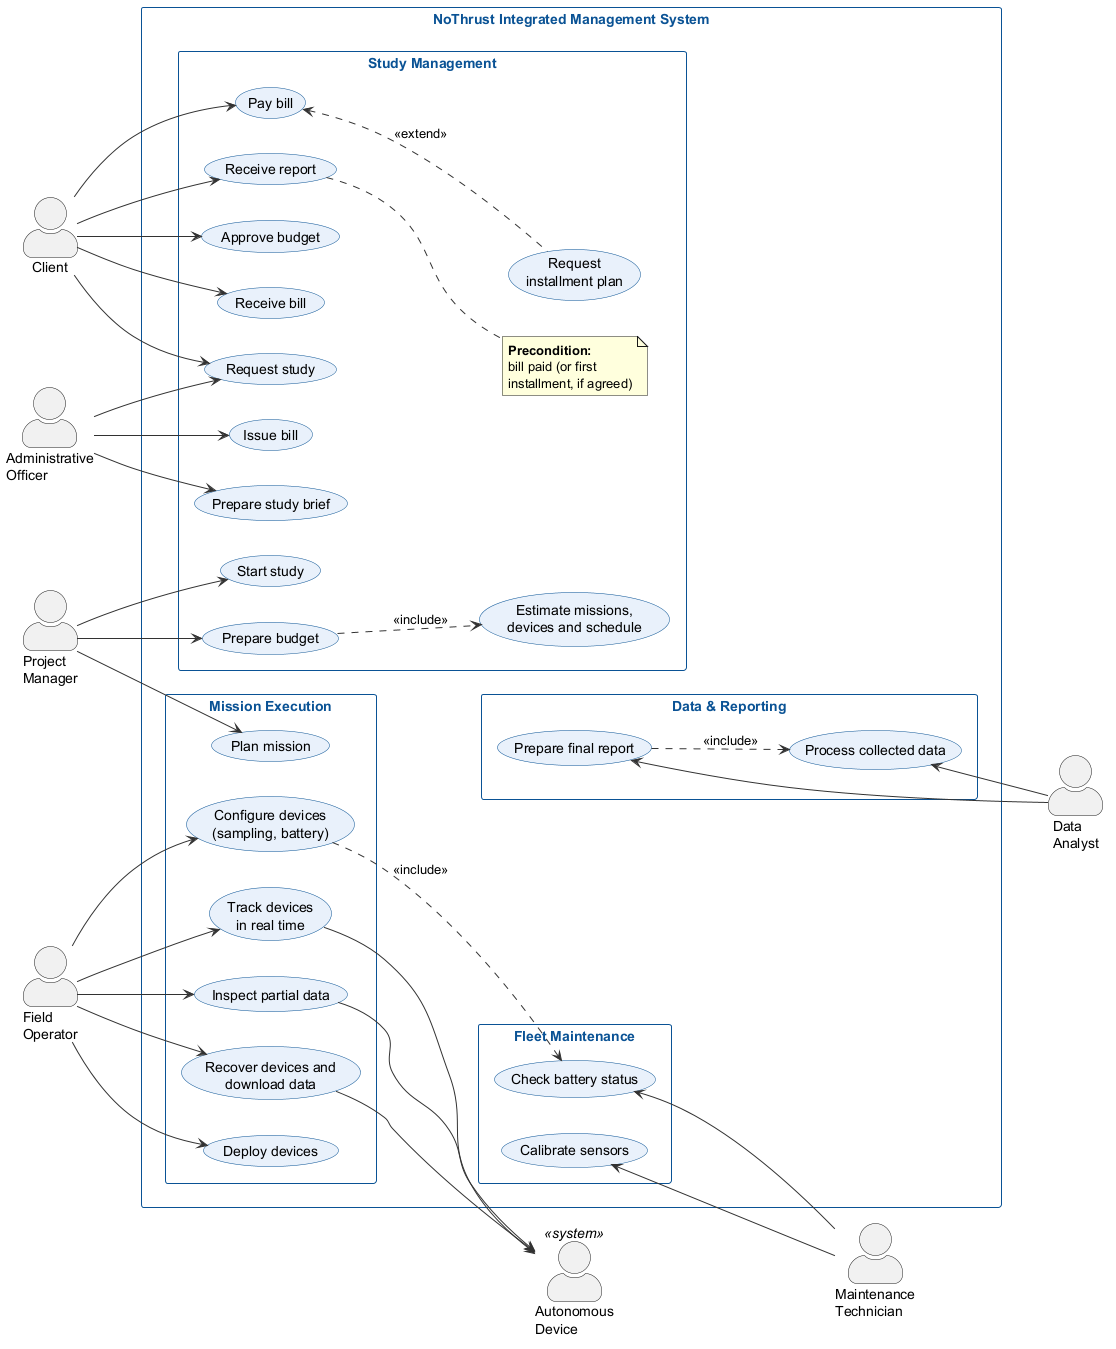
\includegraphics[width=0.72\textwidth]{casos_de_uso.png}
  \caption{Preliminary use case diagram of the NoThrust Inc. system.}
  \label{fig:casos_uso}
\end{figure}

\subsection{Project Workflow}

Figure~\ref{fig:flujo} describes, at a high level, the end-to-end workflow
of a study. Each swimlane corresponds to one of the actors in
Figure~\ref{fig:casos_uso}, and each activity maps to one of its use cases.
The data capture missions are modelled as a loop, since a study may require
one or several missions, and the final report is only delivered once the
bill (or its first installment) has been paid.

\begin{figure}[H]
  \centering
  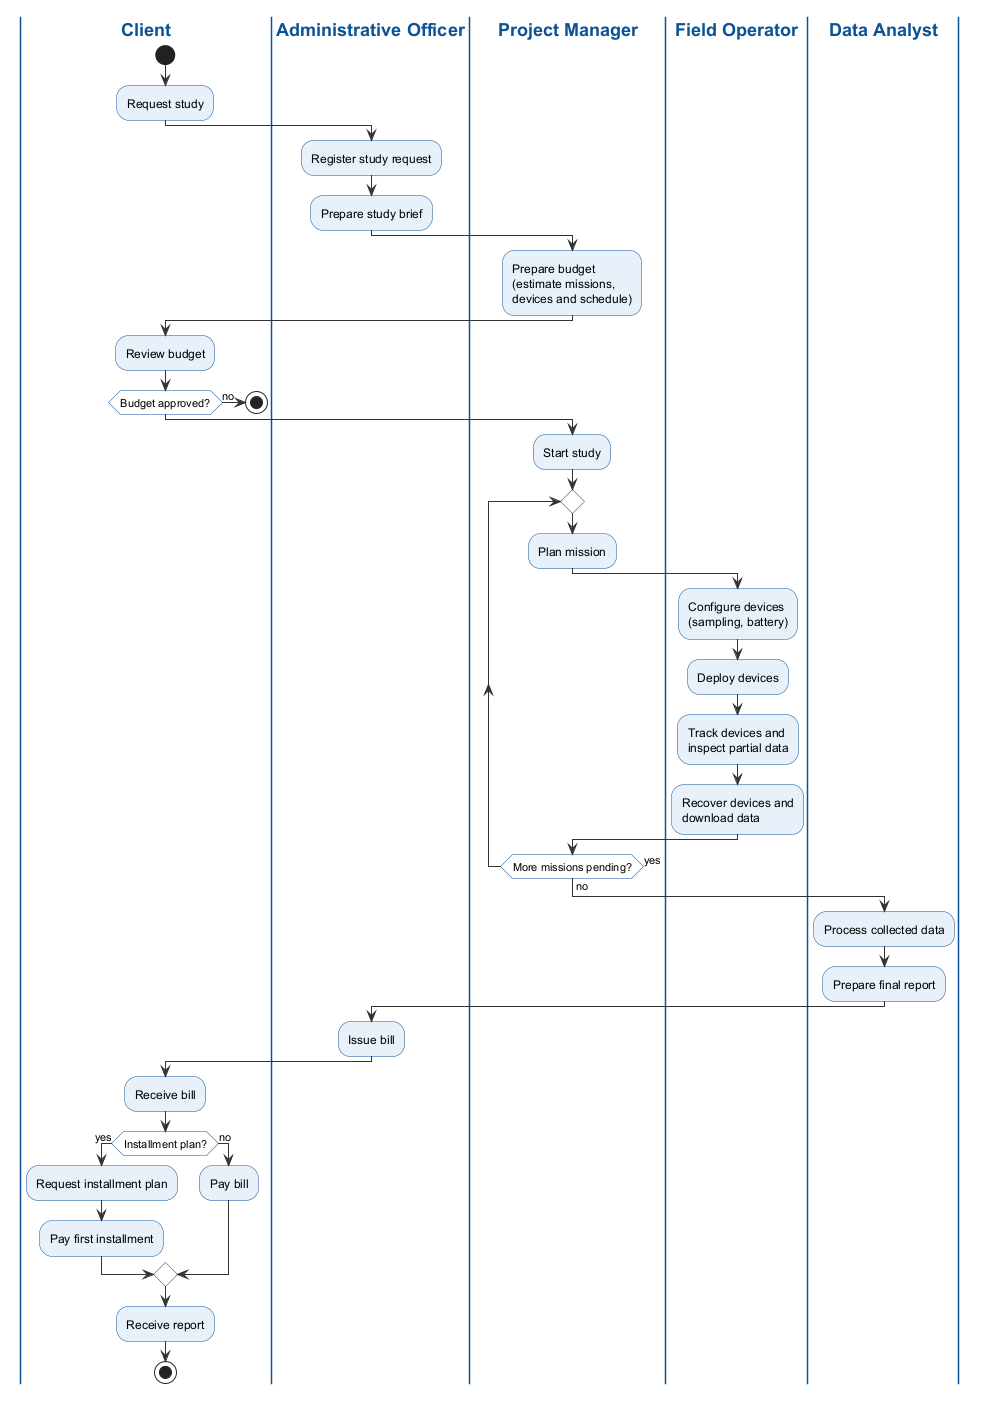
\includegraphics[height=0.6\textheight,keepaspectratio]{basic_proyect_flow.png}
  \caption{High-level activity diagram of a study, from request to report delivery.}
  \label{fig:flujo}
\end{figure}

\section{Conclusions}

The analysis presented identifies seven actors, four functional areas and
the end-to-end workflow of a study, from the client's request to the
delivery of the report and the bill. The requirements show that the system
is not only a fleet control tool, but an integrated platform where
commercial, operational and maintenance activities share the same data,
which will require careful attention during the modeling phase.
The non-functional requirements, especially real-time telemetry, tolerance
to intermittent links and the integration of new device types, will be
the main drivers of the architecture in the design phase.
Overall, these aspects show that the success of the project will depend on
a large team with specialised expertise in the technologies involved.

\end{document}
